\documentclass[a4paper,12pt,oneside]{report}
\usepackage{titlesec}
\usepackage[svgnames]{xcolor}
%\usepackage[usenames,dvipsnames]{color}
\usepackage[top=0cm,bottom=0cm,left=0cm,right=0cm]{geometry}
%\usepackage{fullpage}
\usepackage[utf8]{inputenc}
\usepackage[T1]{fontenc}
\usepackage{graphicx}
\usepackage{wallpaper}
\usepackage{wrapfig}
\usepackage{hyperref}
\usepackage[francais]{babel}
%\usepackage{color}
\usepackage{layout}
\usepackage{circuitikz}
\usepackage[squaren, Gray]{SIunits}
\usepackage{sistyle}
\usepackage[autolanguage]{numprint}

%Algo package
\usepackage[ruled,vlined]{algorithm2e}
\usepackage{algpseudocode}

\usepackage{array}
\usepackage{calc}

\hypersetup{pdfborder={0 0 0}}

\titleformat{\part}
{\centering\fontfamily{pag}\fontsize{30}{30}\selectfont}
{\fontfamily{pag}\fontsize{30}{30}\selectfont Partie \ \thepart \ - }
{0pt}
{}{}

%Modifie le format des chapitres
\titleformat{\chapter}
{\it \color{DodgerBlue} \fontfamily{pag}\fontsize{20.74}{20}\selectfont}
{\it \fontfamily{pag}\fontsize{20.74}{20}\selectfont Chapitre \ \thechapter \ - }
{0pt}
{}{}
\titlespacing{\chapter}{0pt}{0.5cm}{0.5cm}[0pt]

%Modifie le format des sections
\titleformat{\section}
{\color{LimeGreen}\fontfamily{pag}\fontsize{15}{15}\selectfont}
{\fontfamily{pag}\fontsize{15}{15}\selectfont \thesection }
{5pt}
{}{}
\titlespacing{\section}{1cm}{0.5cm}{0.25cm}[0cm]

%Modifie le format des sous-secions
\titleformat{\subsection}
{\color{DarkOrange}\fontfamily{pag}\fontsize{12}{12}\selectfont}
{\fontfamily{pag}\fontsize{12}{12}\selectfont \thesubsection}
{5pt}
{}{}
\titlespacing*{\subsection}{2cm}{0.1cm}{0.1cm}[0cm]

%Modifie l'espace avant les paragraphes
\setlength{\parindent}{0pt}
\makeatletter

\newcommand{\bigO}{$\mathcal{O}$}

% Commande créeant une page de titre
%	#1=Titre
%	#2=Sous-titre
%	#3=Auteur
%	#4=image
%	#5=couleur de fond
%	#6=couleur cadre titre,sous-titre,auteur
\newcommand{\titre}[6]
{
	\begin{document}
	\begin{titlepage}
		\pagecolor{#5} % met la couleur de la page
		\vspace*{0.6cm}\fontfamily{pag}\fontsize{20}{20}\selectfont{\begin{center}2015-2016\end{center}}\vspace*{0.3cm}	% insère l'année en haut de la page
		\vspace*{-0.1cm}
		\includegraphics[width=\paperwidth]{#4} % insère l'image
		\colorbox{#6}{	%boîte de couleur avec le titre, sous-titre et l'auteur
			\hspace*{1.2cm}
			\begin{minipage}{\textwidth-1.8cm}{
				\vspace*{1cm}
				\begin{flushleft}\bfseries
					\fontfamily{pag}\fontsize{35}{35}\selectfont{#1}	%Titre
					\vspace*{0.5cm}
				\end{flushleft}
				\begin{flushleft}
					\fontfamily{pag}\fontsize{30}{30}\selectfont{#2}	%Sous-Titre
				\end{flushleft}
				\vspace*{1cm}
				\begin{flushright}
					\fontfamily{pag}\fontsize{20}{20}\selectfont{#3}	%Auteur
				\end{flushright}}
			\vspace*{1cm}
			\end{minipage}}
			\begin{center}
				\vfill % repli le reste de la page
				\fontfamily{pag}\fontsize{20}{20}\selectfont{\today} 	%Date
			\end{center}
	\end{titlepage} % fin de la page de titre
	\color{black} % met la couleur du reste du texte à noir
	\pagecolor{white}	% met la couleur des pages suivante à blanc
	\newgeometry{top=1.5cm,bottom=1.5cm,left=1cm,right=1cm}	% modification des marges
	\tableofcontents	%tables des matières
}
\titre{SINF-1121 Algorithmique et structures de données}{Synthèse}{Damien Deprez}{PageDeGarde}{LightBlue}{LightGreen}
\chapter{Algorithme de Tri}
\section{Selection Sort}
L'algorithme de selection sort consiste à chercher dans le tableau le premier plus petit élément et le placer à la première place du tableau. Répéter l'opération pour le deuxième plus petit élément et ainsi de suite. La complexité de cet algorithme est en \bigO$(N^2)$.
 
\begin{algorithm}
 \SetAlgoLined
 \KwIn{$T$ est un tableau de taille $N$}
 \KwResult{Trie le tableau $T$}
 \For{ i de 0 à N-1}
 {min $\leftarrow$ i\\
  \For{j de i+1 à N-1}
  {
  \If{$T$[j] < $T$[min]}
  {
  min $\leftarrow$ j
  }
 }
 \If{min $\neq$ i}
 {
 $T$[i] $\leftrightarrow$ $T$[min]
 }
 }
 \caption{Selection Sort}
\end{algorithm}

\section{Insertion Sort}
L'algorithme d'insertion sort consiste à parcourir le tableau une fois. Si l'élément $i$ est plus petit que celui à la position $i-1$, alors on le fait avancer jusqu'à ce qu'il soit plus grand où égal à l'élément $i-j$. La complexité de cet algorithme est en \bigO$(N^2)$ dans le pire cas. Dans le meilleur cas, c'est en \bigO$(N)$.
\begin{algorithm}
 \SetAlgoLined
 \KwIn{$T$ est un tableau de taille $N$}
 \KwResult{Trie le tableau $T$}
 \For{ i de 0 à N-1}{
 j $\leftarrow$ i\\
 \While{ j > 0 et $T$[j-1] $\geq$ $T$[i]}{
  $T$[j] $\leftrightarrow$ $T$[j-1]\\
  j$\leftarrow$ j-1}
  }
 \caption{Insertion Sort}
\end{algorithm}

\section{Shell Sort}
L'algorithme de Shell Sort est une amélioration de l'algorithme d'Insertion Sort. Le Shell Sort parcours plusieurs fois le tableau mais compare l'élément de la position $i$ avec celui de la position $i-g$ avec $g$ un écart fixé (petit par rapport à la taille du tableau). Chaque parcours de tableau, $g$ diminue pour atteindre 1 à la fin. La complexité de cet algorithme dépends de la séquence de $g$ prise. La séquence 1, 4, 13, 40, 121, 364 donne une complexité de \bigO $(N^{3/2})$. 
\begin{algorithm}
 \SetAlgoLined
 \KwIn{$T$ est un tableau de taille $N$}
 \KwResult{Trie le tableau $T$}
 h $\leftarrow$ 1\\
 \While{h<N/3}{h $\leftarrow$ 3*h+1}
 \While{h $\geq$ 1}{
 \For{ i de h à N-1}{
 j $\leftarrow$ i\\
 \While{ j $\geq$  h et $T$[j-h] $\geq$ $T$[i]}{
  $T$[j] $\leftrightarrow$ $T$[j-h]\\
  j$\leftarrow$ j-h}
  }
  h $\leftarrow$ h/3
  }
 \caption{Shell Sort}
\end{algorithm}
\section{Merge sort}
L'algorithme de Merge Sort est basé sur le principe de \emph{Diviser pour régner}. L'opération principale de cet algorithme est donc de fusionner deux tableaux triés en un seul. Cet étape ce fait en temps linéaire. On effectue donc cette fusion sur les deux moitiés du tableau entré et ainsi de suite. La complexité de cet algorithme est en \bigO $(N\log(N))$. 
\begin{algorithm}
 \SetAlgoLined
 \SetKwProg{Fn}{Function}{}{end}
 \SetKwFunction{MergeSort}{MergeSort}
 \SetKwFunction{size}{size}
 \Fn{\MergeSort{$T$}}{
 \KwIn{$T$, un tableau de taille $N$}
 \KwData{$R$, un tableau vide de taille $N$}
 \KwOut{$R$, un tableau trié de taille $N$}
 \If{$N$>1}{
 A $\leftarrow$ \MergeSort{$T$[ 0,...,$N$/2]}\\
 B $\leftarrow$ \MergeSort{$T$[$N$/2+1,...,$N-1$]}\\
 a $\leftarrow$ 1\\
 b $\leftarrow$ 1\\
 \For{i de 0 à N-1}{
  \eIf{(a $\geq$ \size{A} et b > \size{B}) ou A[a] $\geq$ B[b]}{R[i] $\leftarrow$ A[a]\\ a $\leftarrow$ a+1}
  {R[i] $\leftarrow$ B[b]\\ b $\leftarrow$ b+1}
  }
 }
 \Return $R$
 }
 \caption{Merge Sort}
\end{algorithm}
\newpage
\section{Quick Sort}
L'algorithme de Quick Sort est basé sur le principe de \emph{Diviser pour régner}. L'opération principale de cet algorithme est de partitionner un tableau en deux autour d'un éléments appelé le pivot. Ensuite, on recommence l'opération sur les deux tableaux obtenus. Le pivot peut-être choisi de manière aléatoire dans intervalle 0 $N$. La complexité de cet algorithme est en \bigO$(N\log(N))$. 
\begin{algorithm}
 
 \SetAlgoLined
 \SetKwProg{Fn}{Function}{}{end}
 \SetKwFunction{QuickSort}{QuickSort}
 \SetKwFunction{size}{size}
 \SetKwFunction{Random}{Random}
 \Fn{\QuickSort{$T$, $lo$, $hi$}}{
 \KwIn{$T$, un tableau de taille $N$}
 \KwIn{$lo$ entier index de début du tableau}
 \KwIn{$hi$ entier index de fin du tableau}
 \If{lo<hi}{
  pivot $\leftarrow$ \Random{lo,hi}\\
  $T$[pivot] $\leftrightarrow$ T[hi]\\
  j $\leftarrow$ lo\\
  \For{ i de lo à hi-1}{
  \If{T[i] $\leq$ T[hi]}{
  $T$[i] $\leftrightarrow$ $T$[j]\\j $\leftarrow$ j+1}
  }
  $T$[hi] $\leftrightarrow$ $T$[j]\\
  pivot $\leftarrow$ j\\
  \QuickSort{$T$, $lo$, $pivot-1$}\\
  \QuickSort{$T$, $pivot+1$, $hi$}\\
 }
 }
 \caption{Quick Sort}
\end{algorithm}
\chapter{Algorithme de Recherche}
\section{Recherche Séquentielle}
L'algorithme de recherche séquentielle permet de trouver une clé dans une table de symbole non-triée représentée par une liste chaînée. Cette recherche scanne toutes les clés de la table de symbole jusqu'à trouver celle qui est recherchée. La complexité de cet algorithme est en \bigO$(n)$.
\section{Recherche Binaire}
L'algorithme de rechercher binaire permet de trouver une clé dans une table de symbole tirée représentée par un tableau. Si l'élément est plus grand que la clé située au milieu du tableau, alors il se trouve dans le sous tableau de gauche sinon, il se trouve dans le sous tableau de droite. On recommence l'opération de comparaison en déplaçant les indices début, milieu et fin au bord du bon sous tableau. Si l'indice de fin et plus petit que l'indice de début du tableau c'est que l'élément ne se trouve pas dedans. La complexité de cet algorithme est en \bigO$(\log(n))$.
\section{Structure de données pour les Tables de Symboles}
\subsection{Arbres binaires}
La représentation sous forme d'arbre binaire une table de symboles permet d'allier la flexibilité des listes chaînées dans l'ajout et la suppression d'élément et la rapidité de la recherche binaire. La recherche dans un arbre binaire dépends de la forme de l'arbre. Si l'arbre est équilibré, la rechercher est en \bigO$(\log(n))$. Si l'arbre n'est pas équilibré, le pire cas est en \bigO$(n)$. La forme de l'arbre dépend de l'ordre d'insertion des clés.
\subsection{Arbres balancés}
L'avantage de l'arbre balancés par rapport à l'arbre binaire est une garantie d'une complexité de recherche en \bigO$(\log(n))$. Pour ce faire, on va utiliser un arbre 2-3.  Chaque nœud de l'arbre 2-3 est soit constitué d'une clé et deux liens vers deux autres nœuds fils (\emph{2-Node}), soit de 2 clés avec trois liens vers des trois autres nœuds fils (\emph{3-Node}). Dans le cadre de trois 3 liens, le lien du milieu veut dire que ce qui est en dessous est entre la clé 1 et la clé 2.\\
\textbf{Insertion}\\
\begin{tabular}{cccc}
\emph{2-Node} &  \emph{3-Node} &  \emph{3-Node} parent \emph{2-Node} &\emph{3-Node} parent \emph{3-Node}\\
\raisebox{1ex-\height}{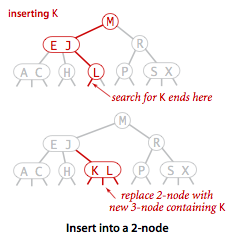
\includegraphics[width=4cm]{23tree-insert2}}&
\raisebox{1ex-\height}{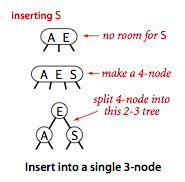
\includegraphics[width=4cm]{23tree-insert3a}} &
\raisebox{1ex-\height}{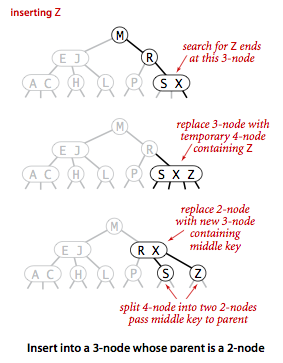
\includegraphics[width=4cm]{23tree-insert3b}} &
\raisebox{1ex-\height}{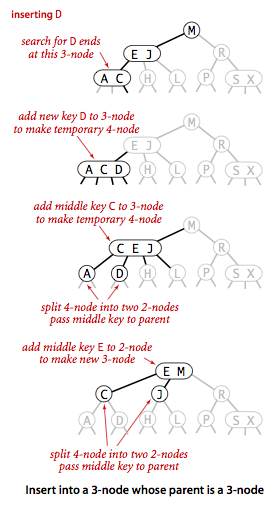
\includegraphics[width=4cm]{23tree-insert3c}}\\
\end{tabular}
Pour représenter un arbre 2-3 sous forme d'arbre binaire simple, on peut utiliser les arbres rouge-noir. Il existe une correspondance immédiate entre les arbres 2-3 et les arbres rouge-noir.
\begin{center}
 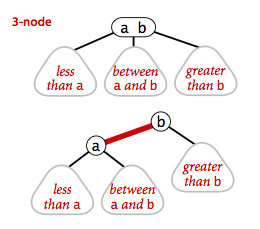
\includegraphics[width=5cm]{redblack-encoding}
\end{center}

\end{document}
